\section{Advantages of Policy Architecture}\label{sec:policy_structure}
In this section, we first evaluate the advantages of the proposed bipedal locomotion control framework in Sec.~\ref{sec:controller} through an extensive ablation study of its design choices. 
This evaluation unfolds from two key perspectives: (1) the learning performance in challenging simulation environments with extensively randomized dynamic parameters, and (2) the control performance during the sim-to-real transfer on a real robot, without any tuning. 
The simulation offers a controlled setting to test the capacity of the control architectures in learning control strategies for large changes in the system dynamics, while real-world experiments allow us to evaluate the control efficacy on the fixed but uncertain dynamics of the robot's hardware. 
As we will demonstrate, our proposed dual-history control architecture and training system result exhibits the best learning performance and sim-to-real transfer. 




\subsection{Baselines}


\begin{figure}[t]
    \centering
    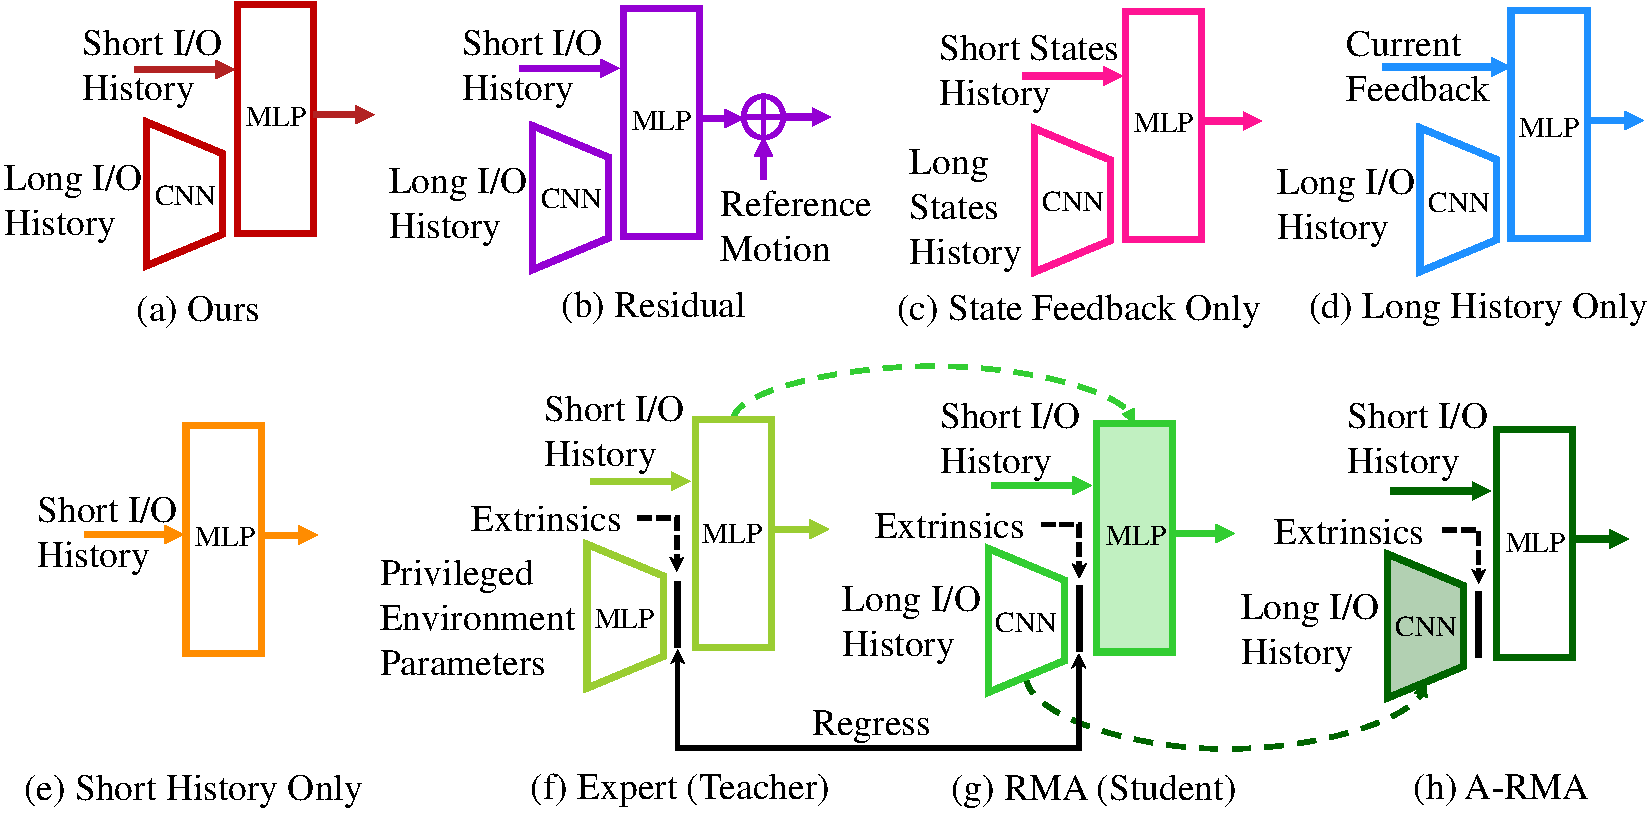
\includegraphics[width=\linewidth]{figures/baselines.pdf}
    \caption{Illustration of our proposed and various baselines for RL-based control policy architectures for bipedal robot locomotion. Fig.~\ref{fig:benchmark}a, \textbf{Ours} integrates both short and long-term I/O histories, with the base MLP and long history encoder jointly trained to specify motor positions. Fig.~\ref{fig:benchmark}b, the \textbf{Residual} approach aligns with our architecture but adds a residual term to the reference motor position. Fig.~\ref{fig:benchmark}c, the \textbf{State Feedback Only} baseline uses our model structure but relies solely on robot's states history, excluding input history. Fig.~\ref{fig:benchmark}d, the \textbf{Long History Only} approach depends on long I/O history without using short I/O history, while the \textbf{Short History Only} approach (Fig.~\ref{fig:benchmark}e) focuses only on short-term I/O history, excluding the CNN encoder. The \textbf{RMA/Teacher-Student} method utilizes a two-phase policy distillation, with an expert (teacher) policy (Fig.~\ref{fig:benchmark}f) guiding the training of an RMA (student) policy (Fig. \ref{fig:benchmark}g), which can be improved by \textbf{A-RMA} (Fig.~\ref{fig:benchmark}h) which introduces an additional phase where the base MLP is finetuned while keeping the long I/O history encoder's parameters fixed. Notably, all expert, RMA, and A-RMA policies in this study incorporate short I/O histories into the base MLP, which is a new modification in this work to enable equitable comparison with ours. All of these architectures have the command and reference motion as input to the base MLP, as detailed in Fig.~\ref{fig:controller} and omitted for brevity.}
    \label{fig:benchmark}
\end{figure}


\begin{figure*}[!htp]
    \centering
    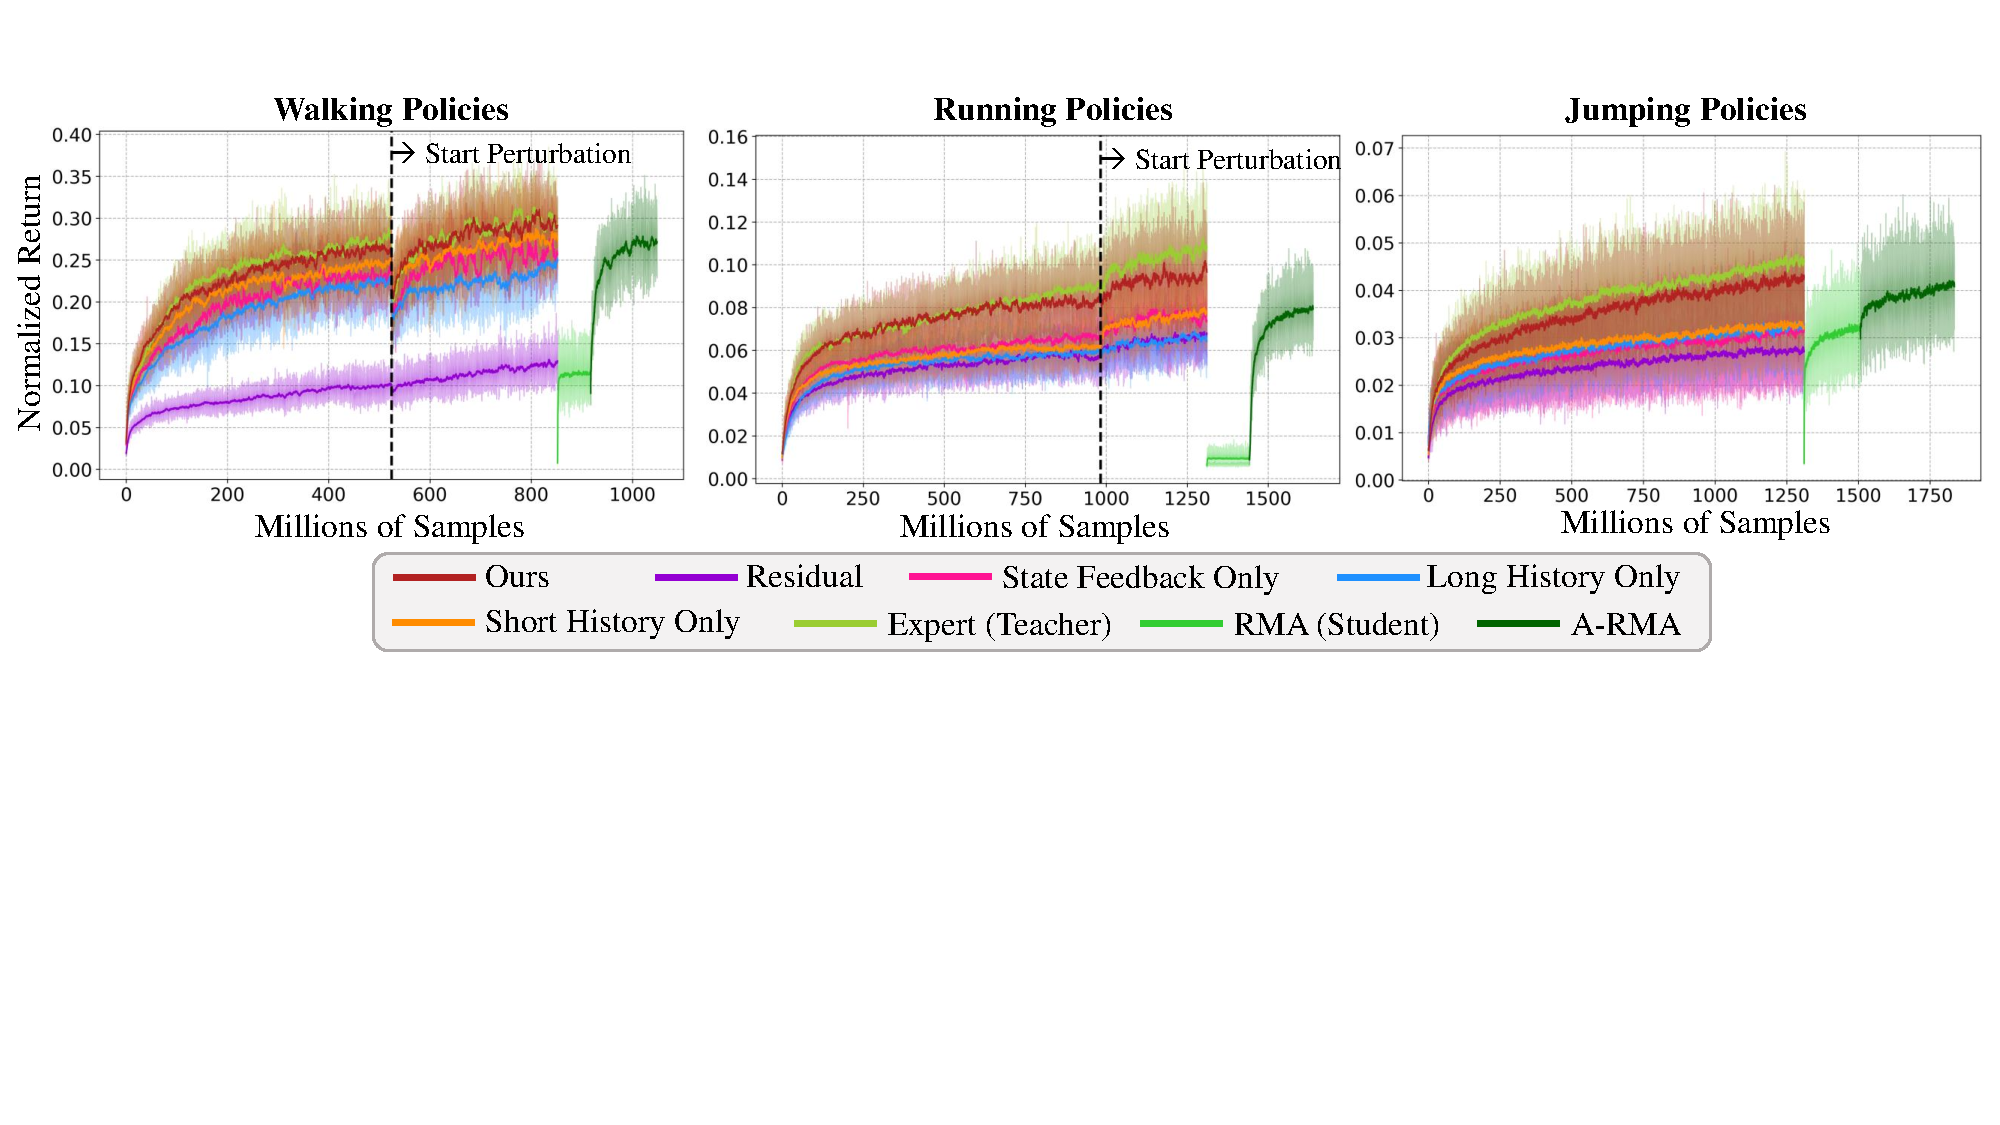
\includegraphics[width=\linewidth]{figures/dynrand_logs_allthree.pdf}
    \caption{The learning performance using different policy structure designs illustrated in Fig.~\ref{fig:benchmark}. It is assessed during Stage 3 training, which incorporates both task and dynamics randomization. These curves represent the average normalized episodic return across 3 distinct policy trainings from different random seeds, with shaded regions indicating the range between minimum and maximum returns. Note that there is no perturbation training for the jumping policy as it prevents the robot from learning the dynamic jumping skill. Our proposed method consistently outperformed other baselines across different skills. Notably, our policy's performance is comparable to that of the expert policy, which has access to privileged information but is not deployable in the real world. In contrast, the residual method shows the worst return. Using only a long history does not offer a clear benefit compared to a policy relying solely on a short history. In fact, the short history only policy even outperforms the long history only approach. Additionally, even with a dual-history approach like ours, omitting the robot's input history (only using state feedback) results in no improvement over short I/O history only. The student or RMA methods exhibit significant regression loss in bipedal locomotion control; particularly in dynamic skills like running, RMA fails to learn. This suggests the necessity of the A-RMA stage for further training, though it requires considerably more training samples and yields slightly lower returns compared to our method. }
    \label{fig:dynrand_three}
\end{figure*}




We compare the proposed controller structure and other baselines listed below and illustrated in Fig.~\ref{fig:benchmark}. Those choices of baselines include ablations on several design choices proposed in this work: (1) choices of action space, (2) history of the robot's I/O or state feedback only, (3) history length (long or short history), (4) dual-history or long history only, (5) end-to-end training or policy distillation. 
The models used in the experiment include:
\begin{itemize}[leftmargin=9pt]
    \small
    \item \textbf{Ours} (Fig.~\ref{fig:benchmark}a): 
    as detailed in Fig.~\ref{fig:controller}, our architecture leverages both short-term and long-term I/O history, with the long-term history encoded by a CNN, while the short-term history is directly fed into the base MLP. The CNN and MLP are trained jointly and the policy outputs specify the desired motor positions.
    \item \textbf{Residual} (Fig.~\ref{fig:benchmark}b): 
    this architecture aligns with our proposed one, but it produces an output that represents a residual term that is then added to the reference motor position at the current timestep, \textit{i.e.}, $q^d_m = \mathbf{a}_t + q^r_m(t)$. Such an approach is employed in prior works like~\cite{lee2020learning,xie2020learning,siekmann2020learning}. It is worth noting that the robot “knows" the current reference motor position to add by taking the reference motion as input.
    \item \textbf{State Feedback Only} (Fig.~\ref{fig:benchmark}c):
    this variant retains the same model structure and action space as ours. However, it differs in its observation by relying solely on the historical states (robot's output history), omitting the robot's input history. Such a choice, \emph{without} the use of short history, is more commonly seen in previous work, such as~\cite{lee2020learning,siekmann2020learning,siekmann2021sim,crowley2023optimizing}.
    \item \textbf{Long History Only} (Fig.~\ref{fig:benchmark}d): this policy architecture relies only on a long-term I/O history encoded by the CNN. This configuration serves as a baseline in~\cite{kumar2021rma}. 
    As suggested by~\cite{peng2018sim}, the base MLP has direct access to the robot's immediate (last-timestep) state feedback. For brevity, in this work, \emph{Long History Only} refers to the method that provides the lastest observation (state feedback) along with the long history encoder, which can be modeled using different neural network architectures.
    \item \textbf{Short History Only} (Fig.~\ref{fig:benchmark}e): this policy relies solely on short-term I/O history, excluding the long-term I/O history CNN encoder. This is used for bipedal locomotion control in~\cite{li2021reinforcement} and is more commonly seen in quadruped control like~\cite{huang2022creating,escontrela2022adversarial,feng2023genloco}.
    \item \textbf{RMA/Teacher-Student}: this architecture utilizes the policy distillation method that involves two training phases. First, an expert (teacher) policy (Fig.~\ref{fig:benchmark}f) is trained by RL that has access to privileged environment information (listed in Table~\ref{tab:randomization}). The privileged information is encoded into an $8$D extrinsics vector by an MLP encoder. \emph{This expert (or teacher) policy can only be used in simulation}. Second, the expert policy is employed to \textit{supervise} the training of an RMA (student) policy (Fig.~\ref{fig:benchmark}g). 
    The RMA policy copies the base MLP from the expert policy and only learns to leverage the long I/O history encoder to estimate the teacher's extrinsic vector. 
    Such a policy distillation method is used in~\cite{lee2020learning,kumar2021rma} and widely adopted in quadrupedal locomotion control.
    \item \textbf{A-RMA} (Fig.~\ref{fig:benchmark}h): 
    after the RMA training, an additional training phase is introduced. In this phase, the long I/O history encoder's parameters remain fixed, while the base MLP is updated again through RL, as introduced by~\cite{kumar2022adapting}. 
    \emph{Notably, during the implementation, all expert, RMA, and A-RMA policies incorporate short I/O histories to the base MLP in this study, which is a new modification in this work to enable an equitable comparison with ours.}
\end{itemize}





For each locomotion skill studied in this work (walking, running, and jumping), using our proposed method and baseline methods, we obtained 3 policies trained by the identical multi-stage training framework introduced in Sec.~\ref{sec:training}. These policies were obtained from the same choice of hyperparameters, but from different random seeds. This was done for each of these policy architectures. 
In other words, $3\times3\times8=72$ different control policies are obtained, representing 3 locomotion skills, 3 random seeds, 8 policy architectures, and evaluated below.   








\subsection{Learning Performance}



We begin our evaluation by benchmarking our method against various baselines in simulation by examining their respective learning curves. 
Our focus lies on the training performance during Stage 3, as shown in Fig.~\ref{fig:dynrand_three}, the most challenging stage that involves both randomized tasks and dynamics parameters. 
This particular emphasis on Stage 3 also stems from its critical role in sim-to-real transfer, a pivotal concern within the scope of controlling real bipedal robots in our study. 

\subsubsection{Benchmark Analysis}
As depicted in Fig.~\ref{fig:dynrand_three}, the learning performance remains uniform across various locomotion skills, as outlined and analyzed below. 

\paragraph{Choices of Action}
We observe that when the policy produces a residual term (purple curves) instead of directly specifying the desired motor position, the learning performance consistently deteriorates across various locomotion skills. 
Although the added reference motion to the action might accelerate the learning of the desired skill initially, this added reference motion could also introduce additional movements to the robot. 
Consequently, the policy expends more effort correcting the added movements rather than effectively controlling the robot, which becomes more problematic when the robot explores maneuvers beyond the reference motion. 
Hence, we recommend readers reconsider the use of residual learning in the context of locomotion control, regardless of whether the added action is optimized for dynamic feasibility (as in walking) or limited to kinematic feasibility (as in running or jumping).

We also consider another action space option: joint-level torque. RL has been used to learn torque control for quadrupedal and bipedal robots as demonstrated in~\cite{chen2022learning} and \cite{kim2023torque} respectively. However, torque control's high update frequency requirements, such as 250 Hz in~\cite{kim2023torque}, restrict its ability to utilize extensive robot I/O history. Prior methods using torque control have thus been limited to a single timestep of robot feedback. Later, we will demonstrate that a longer I/O history, like 2 seconds, could improve the adaptivity of RL-based controllers, but recording and learning with such a long history is computationally expensive for high-frequency torque controllers, as the action (robot's input) history needs to update at the same frequency as the controller. Therefore, our benchmark focuses on policies that can operate effectively at lower frequencies.



\begin{figure*}[!htp]
    \centering
    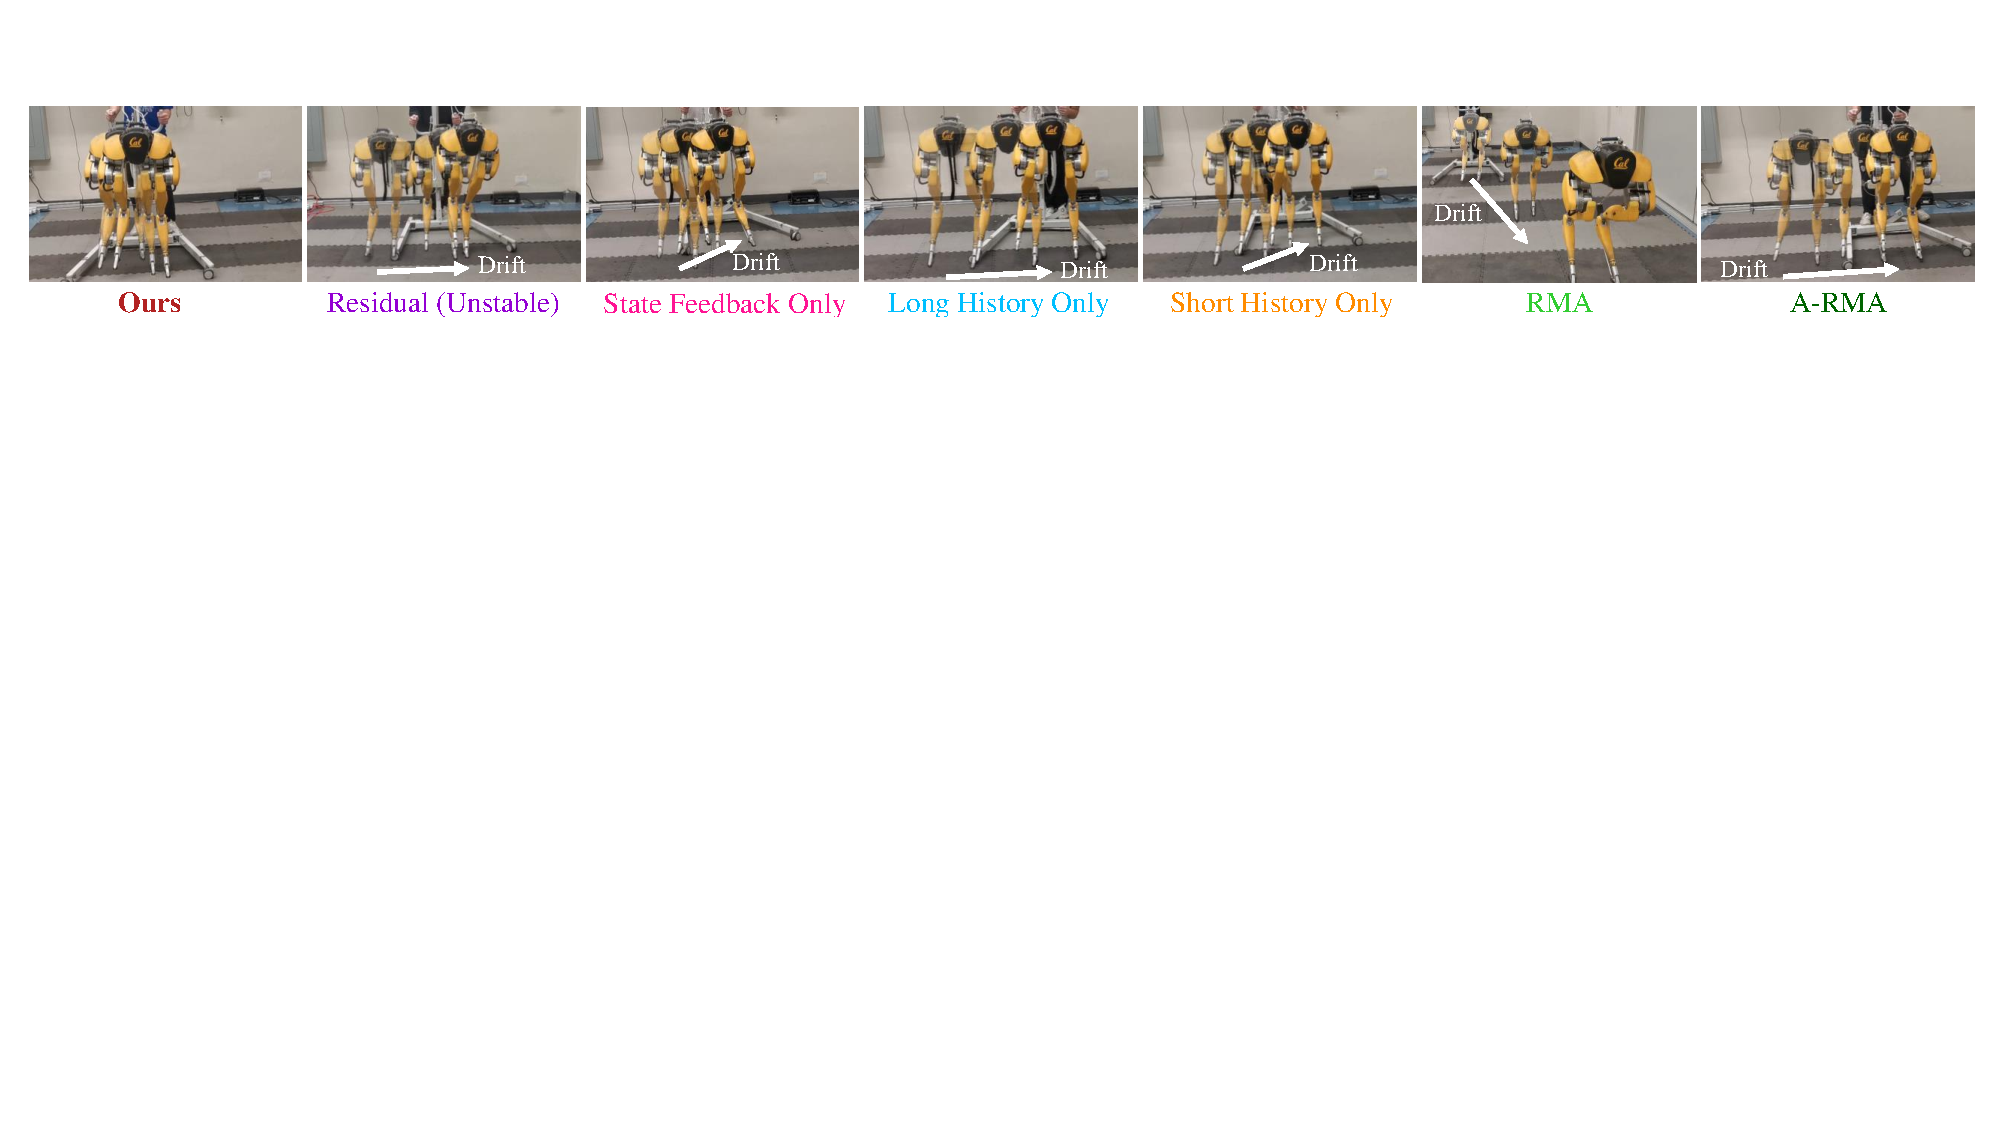
\includegraphics[width=\linewidth]{figures/bm_inplace_realworld.pdf}
    \caption{Snapshots from experiments of the bipedal robot Cassie controlled by different policies trained by different methods illustrated in Fig.~\ref{fig:benchmark}. The test is to control the robot to walk in place, \textit{i.e.}, $(\dot{q}^d_x, \dot{q}^d_y, q^d_{\psi}) = \mathbf{0}$. Each snapshot compiles three frames taken at the \emph{same} 1$^{\text{st}}$, 4$^{\text{th}}$, 7$^{\text{th}}$ second after initialization. Our method exhibits minor drift (the robot does not leave its initial place as demonstrated in the figure), outperforming other approaches, which all result in notable sagittal and/or lateral drifts (marked by the white arrows). Furthermore, the residual policy failed to control the robot to maintain a stable gait. This benchmark underscores the advantages of our proposed architecture in adapting to the real robot's dynamics for better tracking performance after zero-shot transfer. These results are consistent over different policies trained from different random seeds, which are reported in Fig.~\ref{fig:bm_errobar}.}
    \label{fig:bm_realworld}
\end{figure*}


\begin{figure*}[!htp]
    \centering
    \begin{subfigure}{0.49\linewidth}
      \centering
      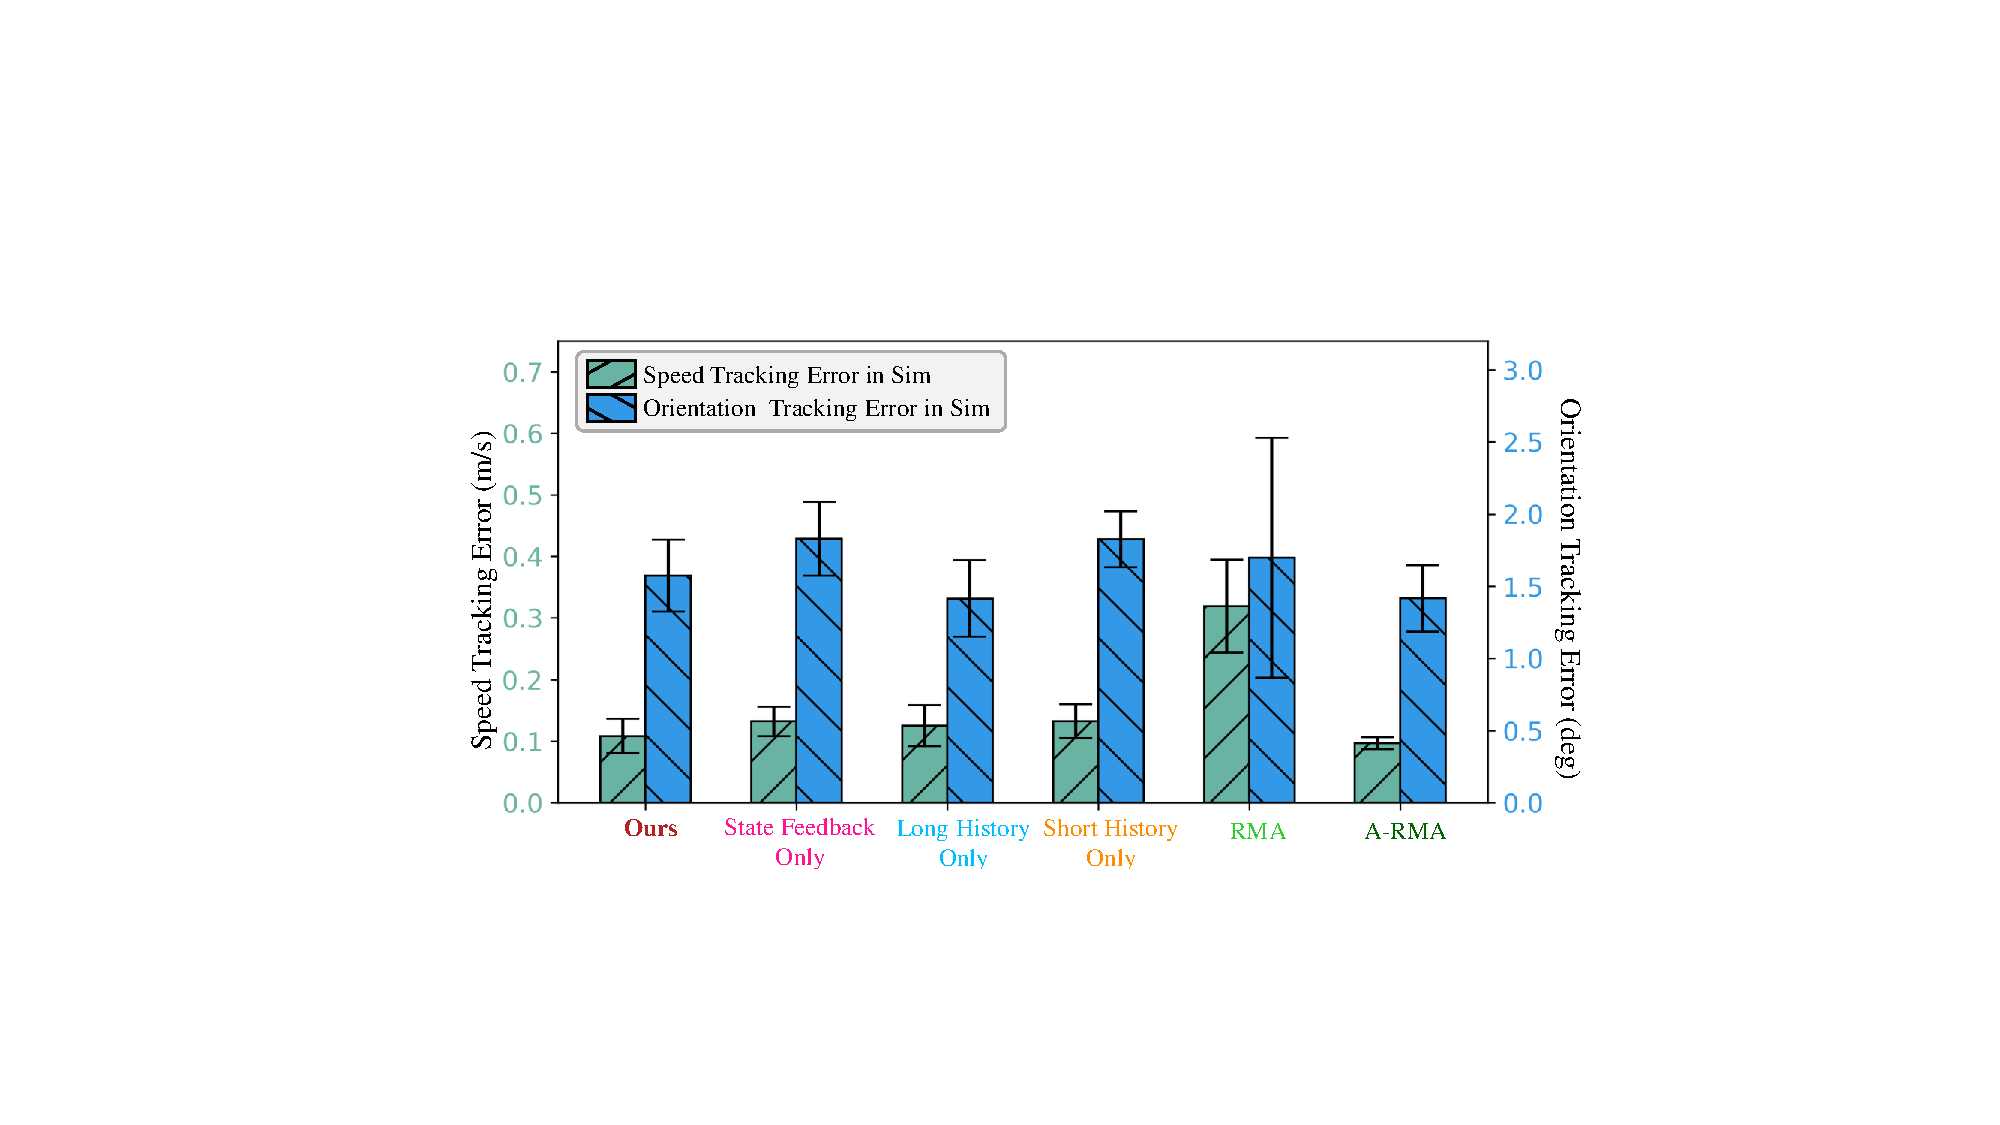
\includegraphics[width=\linewidth]{figures/bm_errorbar_sim.pdf}
      \caption{The bar chart of tracking performance (zero-speed) using the \textit{same} policies tested in the simulation.}
      \label{subfig:bm_errorbar_sim}
    \end{subfigure}    
    \begin{subfigure}{0.49\linewidth}
      \centering
      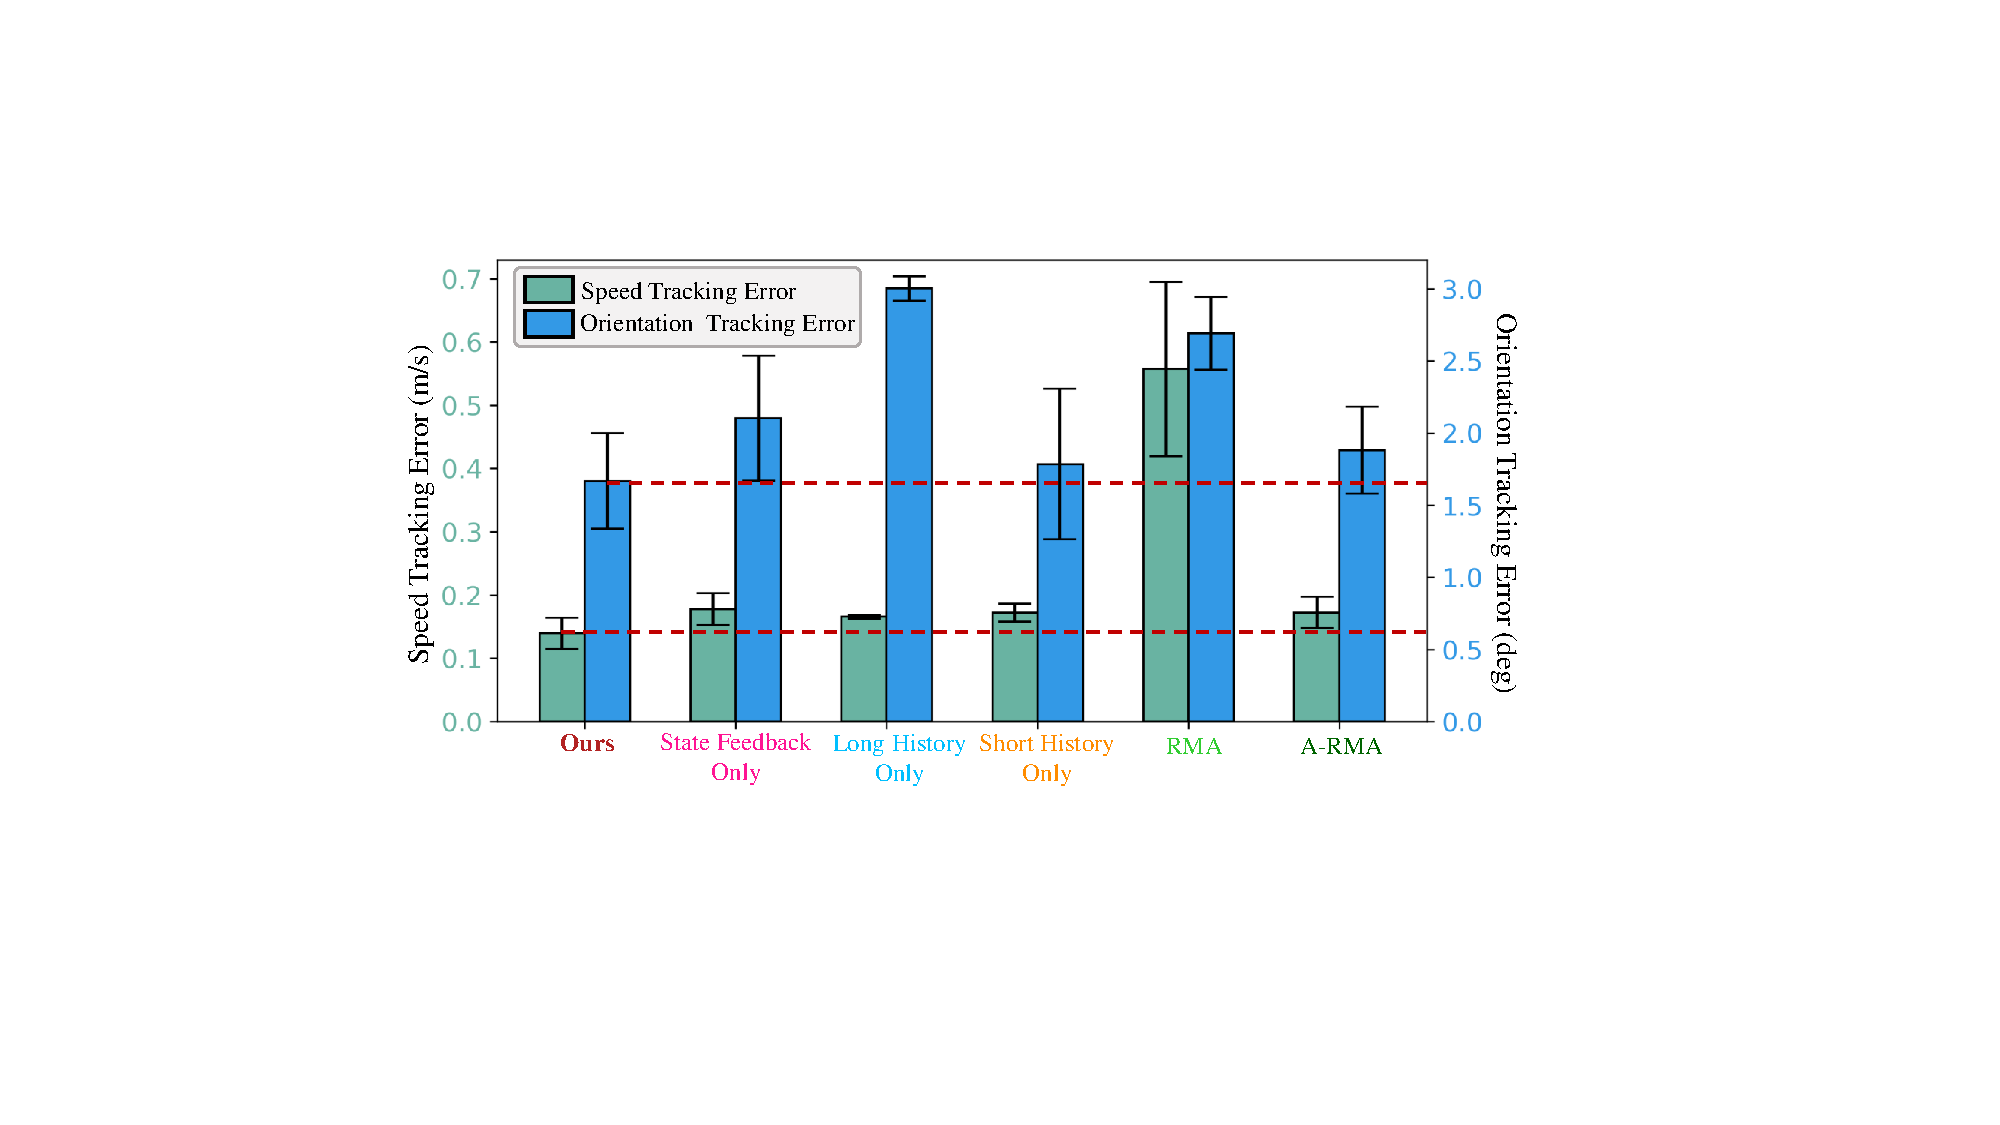
\includegraphics[width=\linewidth]{figures/bm_errorbar_real.pdf}
      \caption{The bar chart of tracking performance (zero-speed) using the obtained walking policies tested on the robot hardware. }
      \label{subfig:bm_errorbar_real}
    \end{subfigure}    
    \caption{The bar chart of the tracking performance using different policies obtained by different methods (Fig.~\ref{fig:benchmark}) in the in-place walking experiments in the simulation (Fig.~\ref{subfig:bm_errorbar_sim}) and the real world (Fig.~\ref{subfig:bm_errorbar_real}). The speed tracking error (Mean Absolute Error, MAE, of $||\dot{q}_{x,y}||_2$) and orientation tracking error (MAE of $q_{\phi,\theta,\psi}$) using the policies trained from \emph{different random seeds} but same method are recorded. They are shown in green and blue bars, respectively. The bar height is the average tracking error over three random seeds and the error bar represents the standard deviation among these three tests. We exclude the residual approach as it can not maintain a stable gait. Training from different random seeds, while all methods perform similarly well in the simulation, when transferring the same policies to the hardware, our method consistently demonstrates the minimal speed tracking error and orientation tracking error over other methods. This underscores the capacity of the proposed method in terms of adapting to the robot dynamics in the real world.}
    \label{fig:bm_errobar}
\end{figure*}




\paragraph{Choices of Observation}
A comparison between our proposed method (red curves), which considers the robot's I/O history, and a baseline that relies solely on the robot's output history (pink curves) reveals an important finding: omitting the robot's input (action) history leads to a decline in learning performance, even with an identical policy architecture and training approach. 
In other words, providing only the history of the robot's state feedback in the observation is insufficient.
This comparison illustrates the critical role of utilizing both the robot's input and output history in developing a control policy through model-free RL.
This combined I/O history is crucial for the control policy to perform system identification and state estimation to infer the robot's system parameters and states, which enhances its adaptivity to uncertain dynamics and external perturbations.
This importance becomes particularly pronounced in our work, where we tackle the control of a highly nonlinear high-dimensional system (bipedal robot) using limited and noisy, delayed measurements (partial observability).


\paragraph{Long History versus Short History}
When leveraging long I/O history alone (blue curves), the learning performance fails to surpass that of the policy utilizing only short I/O history (orange curves) or others.
However, when we provide the base MLP with direct access to the short I/O history while having a long history encoder, as proposed in our approach, the resulting learning performance exhibits significant improvement. 
This enhancement is rooted in the real-time control context, where the short history becomes crucial for information about the robot's very recent I/O trajectory. 
While the long history does contain this short-term information, it can become obscured after passing through an encoder. Hence, providing the policy with direct access to \emph{explicit} short history within the base MLP complements the utilization of long history. Further discussion is presented in Sec.~\ref{subsec:dual_history_advantages}.
Additionally, in Appendix~\ref{appendix:history_length}, we delve into the effects of varying history lengths for temporal encoding. We found that increasing the history length can enhance training performance, but improvements tend to plateau with longer histories and may even hinder training by introducing redundant information for locomotion control. The 2-second history tends to perform consistently well in all the skills developed in this work.


\begin{remark}
   In Appendix~\ref{appendix:lstm_tcn}, we explore the effects of training performance using different temporal encoders such as TCN~\citep{lee2020learning} and LSTM~\citep{siekmann2020learning}. We found that a dual-history approach consistently enhances learning performance for non-recurrent policies like TCN that encode an explicit history length. However, for recurrent policies like LSTM, the dual-history approach does not significantly aid learning. Additionally, recurrent policies tend to converge to more suboptimal policies than non-recurrent ones and are sensitive to hyperparameter tuning across different MDPs (locomotion skills).
\end{remark}

It's important to clarify that our aim is not to dispute the use of a specific temporal encoding structure or the use of a long history. 
Instead, our emphasis lies in underlining the importance of incorporating short history when working with long history data, which can be encoded by many choices of structures.




\paragraph{Comparison with Policy Distillation Methods}
A comparison between our method that jointly trained the long history encoder with the base MLP (red curves) and policy distillation methods that separate the training of the base MLP and history encoder (green curves) highlights the significance of using a right training strategy. 
We observed that the RMA (student) policy exhibits significant degradation compared to the expert policy, primarily due to the unavoidable error when utilizing the robot's long history to estimate pre-selected environment parameters (encoded to the extrinsics vector). 
This decline in RMA's performance becomes particularly prominent when dealing with challenging locomotion skills, such as running, where it fails to learn.
A-RMA, which continues fine-tuning the base MLP with the frozen estimation encoder, can enhance RMA performance but it still falls slightly short when compared to our proposed method, despite having significantly more training samples. 
In the case of running, where the encoder struggles to estimate environment parameters, A-RMA essentially reproduces the result of the short history-only policy (the orange one), avoiding the use of long history.
\emph{It's worth noting that although there are other potential ways to enhance RMA learning like~\cite{fu2023deep}, our proposed method consistently demonstrates performance similar to the expert policy which is the theoretical upper bound for the student policy. Importantly, our approach is deployable in the real world, whereas the expert policy is not.}




\subsection{Case Study: In-place Walking Experiments}
We proceed to conduct a case study on the policies trained using various methods, as depicted in Fig.~\ref{fig:benchmark}, in the real world. 
We choose to assess the walking policies for controlling Cassie to sustain an in-place walking gait in the real world without any tuning or global position feedback.
This relatively straightforward scenario can provide valuable insights into the adaptivity of the trained policies. 
If the policy is unable to adapt to the dynamics of the real robot, it may result in obvious drift, even if it effectively maintains the robot's walking gait.

As shown in Fig.~\ref{fig:bm_realworld}, the results highlight a significant contrast.
Our proposed method demonstrates notably lower tracking errors and successfully maintains the robot's in-place walking, with minimal drift observed in both sagittal and lateral directions. 
Conversely, policies utilizing long history only, short history only, and dual-history with only state feedback, when trained under the same number of samples, result in substantial drift to the robot's left.
Furthermore, RMA demonstrates the most obvious sagittal shift and it walks forward using a fast speed even with a zero velocity command. 
While A-RMA reduces this sagittal drift, it still experiences considerable lateral movement. 
Moreover, the residual policy fails to maintain a stable gait on the real robot.
The corresponding video is recorded in Vid. 3 in Table~\ref{tab:video_list}.

Since we obtained three distinct policies trained from different random seeds, we test each of these policies for the same in-place walking in both the simulation using the robot nominal model and the real world, and compare the statistical results in Fig.~\ref{fig:bm_errobar}.  
The robot's speed ($||\dot{q}_{x,y}||_2$) and base orientation ($q_{\phi,\theta,\psi}$) tracking errors (Mean Absolute Error, MAE) over a 10-second test are evaluated. 
Note that, besides the turning yaw ($q_{\psi}$) that is included in the command, we also evaluate the robot's tracking error for the pelvis (base) roll $q_{\phi}$ and pitch $q_{\theta}$ angles. This is done to see which control policy can better stabilize the robot to a small base roll and pitch movement as they are supposed to be zeros. 
As recorded in Fig.~\ref{subfig:bm_errorbar_sim}, all policies trained by different methods exhibit similar good tracking performance in terms of slow speed (except RMA) and floating-base orientation when commanded to walk in place in simulation. 
However, upon transferring to real hardware (Fig.\ref{subfig:bm_errorbar_real}), other methods exhibit significant speed drift and floating base rotational tracking errors.
For example, the long history only policy shows the worst performance in stabilizing the robot's pelvis with a large floating base orientation, yet it has minimal base oscillation in simulation. A-RMA, while best at maintaining the robot's position in simulation, causes significant drift to the robot's left on real hardware. In contrast, our method achieves better sim-to-real transfer performance with minimal degradation and consistently results in better control performance in terms of command tracking and stabilizing the floating base. This underscores the advantages of our approach in adapting to the dynamics of the robot hardware. 

Consequently, we can conclude that the proposed method excels in bridging the sim-to-real gap, demonstrating better performance in effectively controlling the robot in the real-world environment.




\subsection{Summary of Results}
For achieving dynamic bipedal locomotion skills through RL, the results in this section indicate the following design choices for the control policy structure:\\
(1) Have the policy to directly specify motor-level commands rather than using a residual term;\\
(2) Utilize a history of both the robot's input and output, rather than relying solely on the robot's state feedback;\\
(3) When using the robot's I/O history, favor the inclusion of long-term history, but complement it with short-term history in the base policy for enhanced performance, which leads to a dual-history approach; and\\
(4) Train the base policy and the history encoder in an end-to-end manner, as it yields better performance, reducing training complexity and samples compared to policy distillation methods.

These design choices lead to our proposed policy structures, showcasing consistently best learning performance in simulation across various dynamic locomotion skills and delivering improved control results in the real world.